\documentclass{article}

\title{Práctica 2 de Criptografía y Computación}
\date{}
\author{Carlos Núñez Molina \\ Alessandro Zito \\ Gabriela Antolinez}

\usepackage{titlesec}
\usepackage{graphicx}



\titleformat{\section}
  {\normalfont\large}{\thesection}{1em}{}

\begin{document}
	\maketitle
	\newpage	
	
    \section{Análisis tiempos Factorización}
    
    En esta sección vamos a analizar como tarda el algoritmo de Factorizacion por números grandes. Utilizaremos los tres metodologías que tiene ese algoritmo: Fuerza Bruta, Fermat y Ro de Pollard. Hemos hecho los análisis de frecuencias con números al azar y con números productos de primos. Empezaremos comentando con los números al azar.
    
    
    Empezando con el algoritmo de Fuerza Bruta, sabemos que este algoritmo va intentando hasta que no factoriza el numero. Podemos ver en la primera imagen, como el algoritmo va a tardar mucho desde números de 28 cifras; va a crecer exponencialmente el tiempo que tardará el numero a factorizarse hasta un tiempo que es de \begin{math}                                                                                    10^{2}
                                                    \end{math}
    
    
    
    \begin{figure}[ht!]
        \centering
        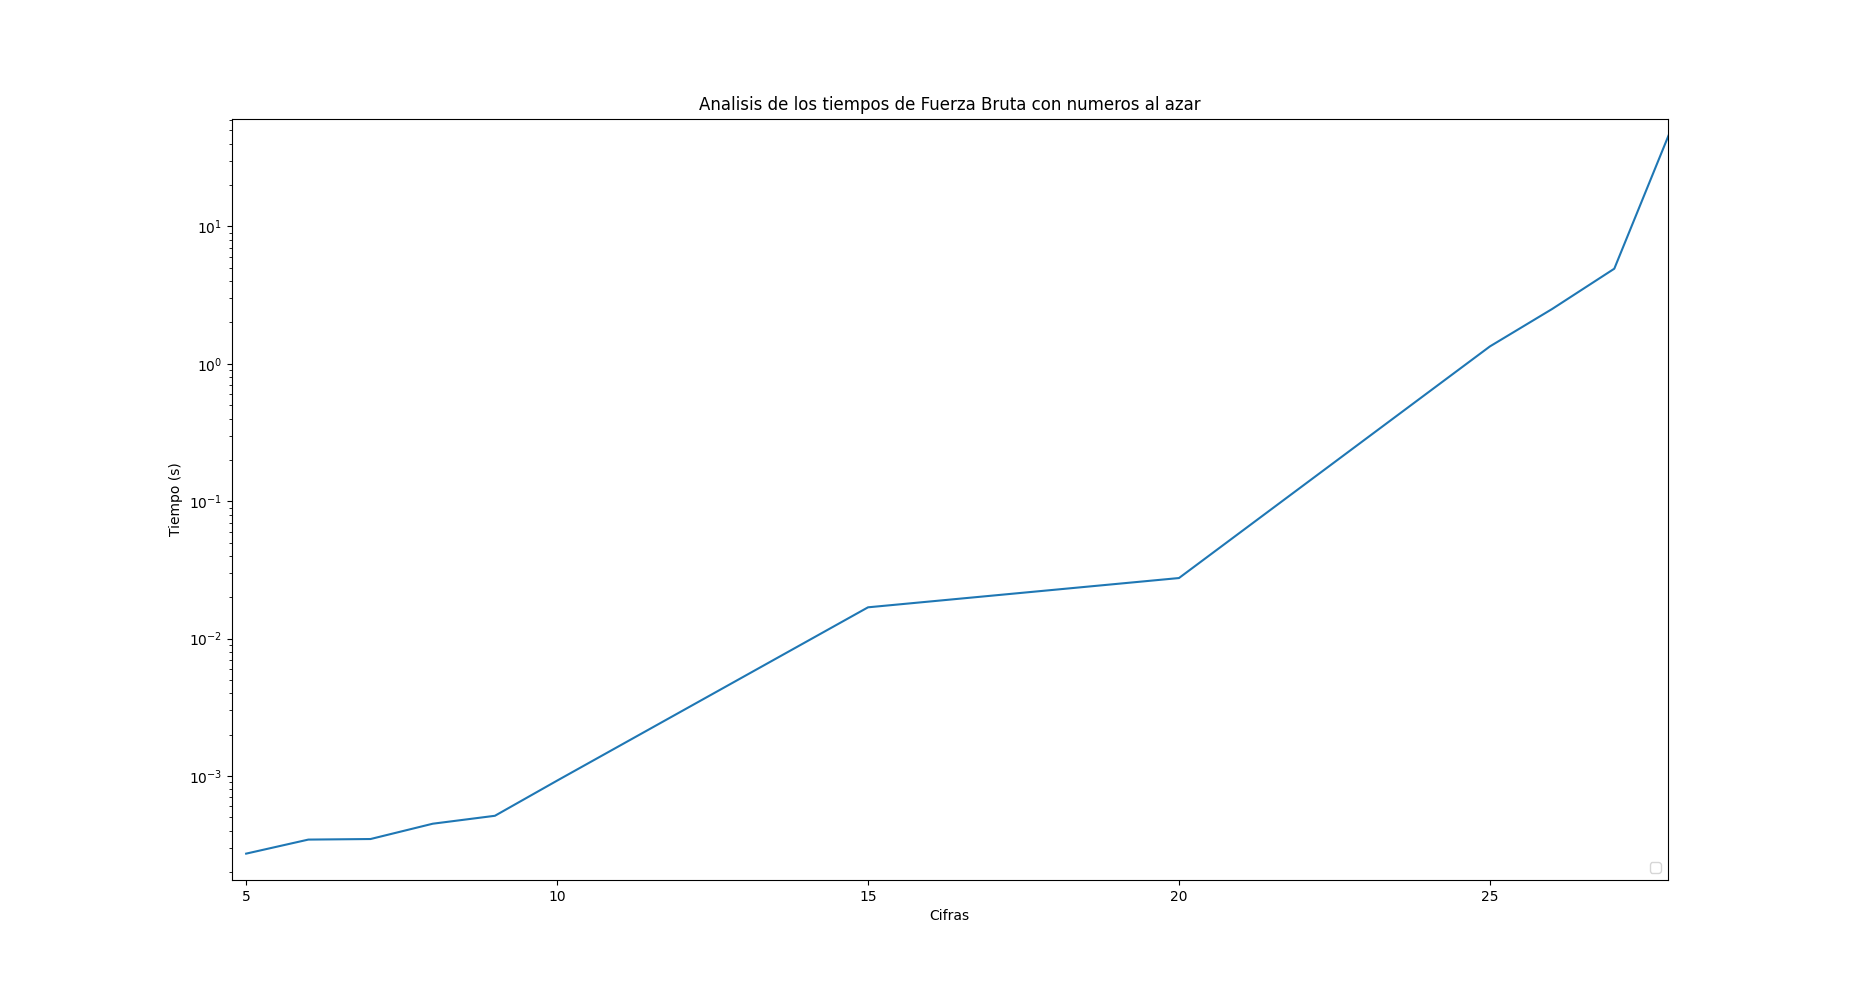
\includegraphics[scale=0.3]{Figure_1}
        \caption{Análisis de los tiempos de Fuerza Bruta con números al azar}
        \label{fig:Figure_1}
    \end{figure}
    
    \newpage
    
     Después siguiendo con el algoritmo de Fermat, sabemos que este algoritmo va a resolver la ecuación \begin{math} y = x ^{2} - n \end{math} para factorizar el numero. Podemos ver en la primera imagen, como el algoritmo va a tardar mucho desde números de 10 cifras; claramente será el peor de los tres, porqué si los factores no son primos, tardará mucho en resolverlo.
    
    
    
    \begin{figure}[ht!]
        \centering
        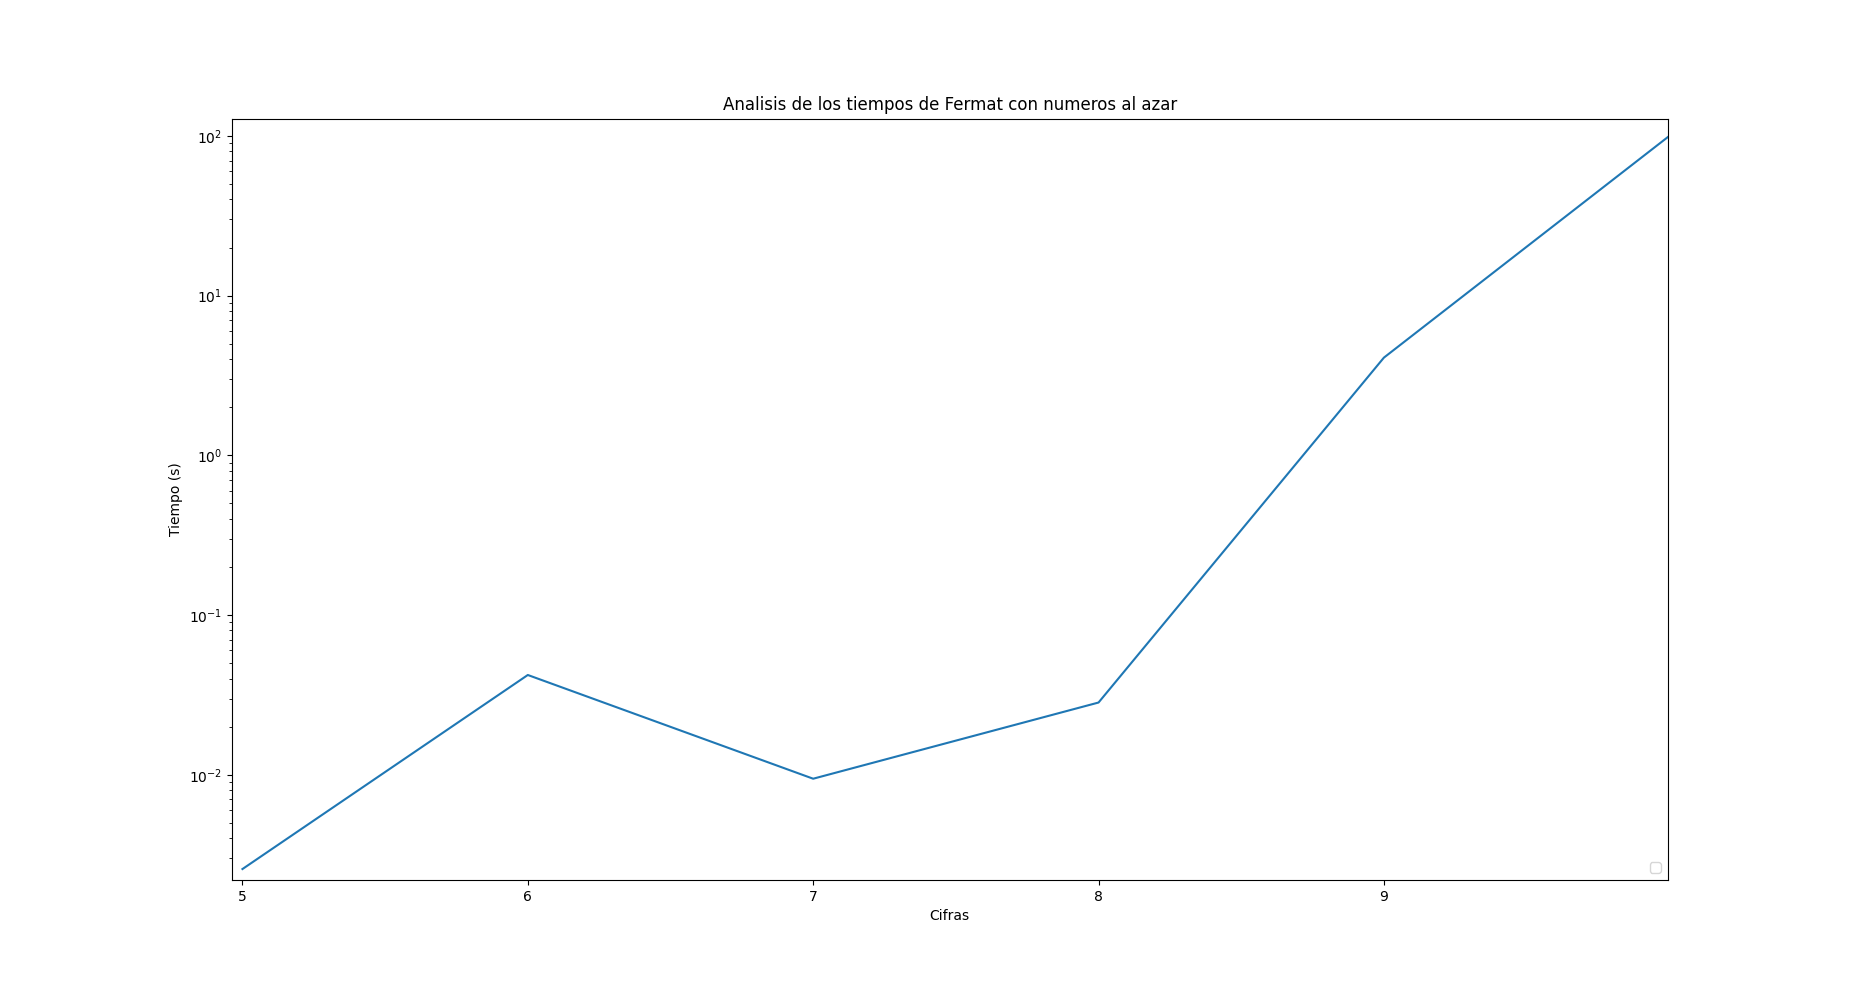
\includegraphics[scale=0.3]{Figure_3}
        \caption{Análisis de los tiempos de Fermat con números al azar}
        \label{fig:Figure_3}
    \end{figure}
    
    \newpage
    
    
    El ultimo de los tres el algoritmo de Ro de Pollard, que tiene el nombre de el matemático que lo inventó. Se trata de construir una sucesión 
    \begin{math}
         x_{1}, x_{2}, ..., x_{n} 
    \end{math} y encontrar dos términos de la sucesión 
    \begin{math} 
        x_{i}, x_{j}
    \end{math} tales que 
    \begin{math}
    mcd(x_{i} - x_{j} ; n) \neq 1.
    \end{math}
    Podemos ver que este algoritmo es el mas eficiente de los 3, porqué se tardará "solo" 100 segundos con numerosa de 42 cifras!
    
    
    \begin{figure}[ht!]
        \centering
        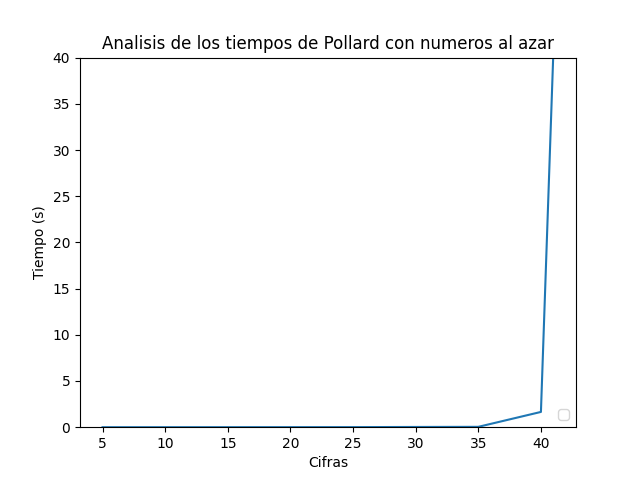
\includegraphics[scale=0.3]{Figure_5}
        \caption{Análisis de los tiempos de Pollard con números al azar}
        \label{fig:Figure_5}
    \end{figure}
    
    
    \newpage
    
    
    Haciendo los mismos test con números productos de dos primos, podemos ver como la eficiencia de Fuerza Bruta y Pollard es menor; sobre todo la de Fermat será mayor; eso porqué Fermat va a buscar los dos factores primos y si son cerca el tiempo será menor.
    
    \begin{figure}[ht!]
        \centering
        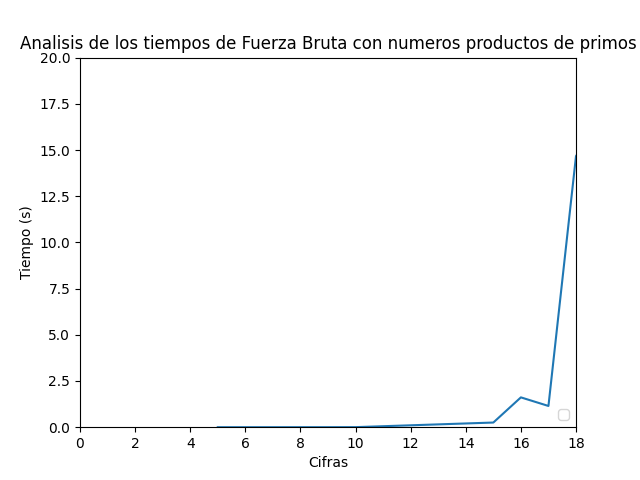
\includegraphics[scale=0.3]{Figure_2}
        \caption{Análisis de los tiempos de Fuerza Bruta con números productos de dos primos}
        \label{fig:Figure_2}
    \end{figure}
    
    \begin{figure}[ht!]
        \centering
        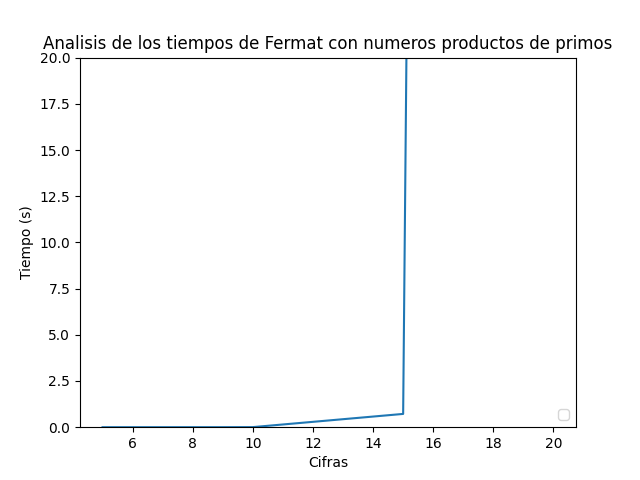
\includegraphics[scale=0.3]{Figure_4}
        \caption{Análisis de los tiempos de Fermat con números productos de dos primos}
        \label{fig:Figure_4}
    \end{figure}
    
    \begin{figure}[ht!]
        \centering
        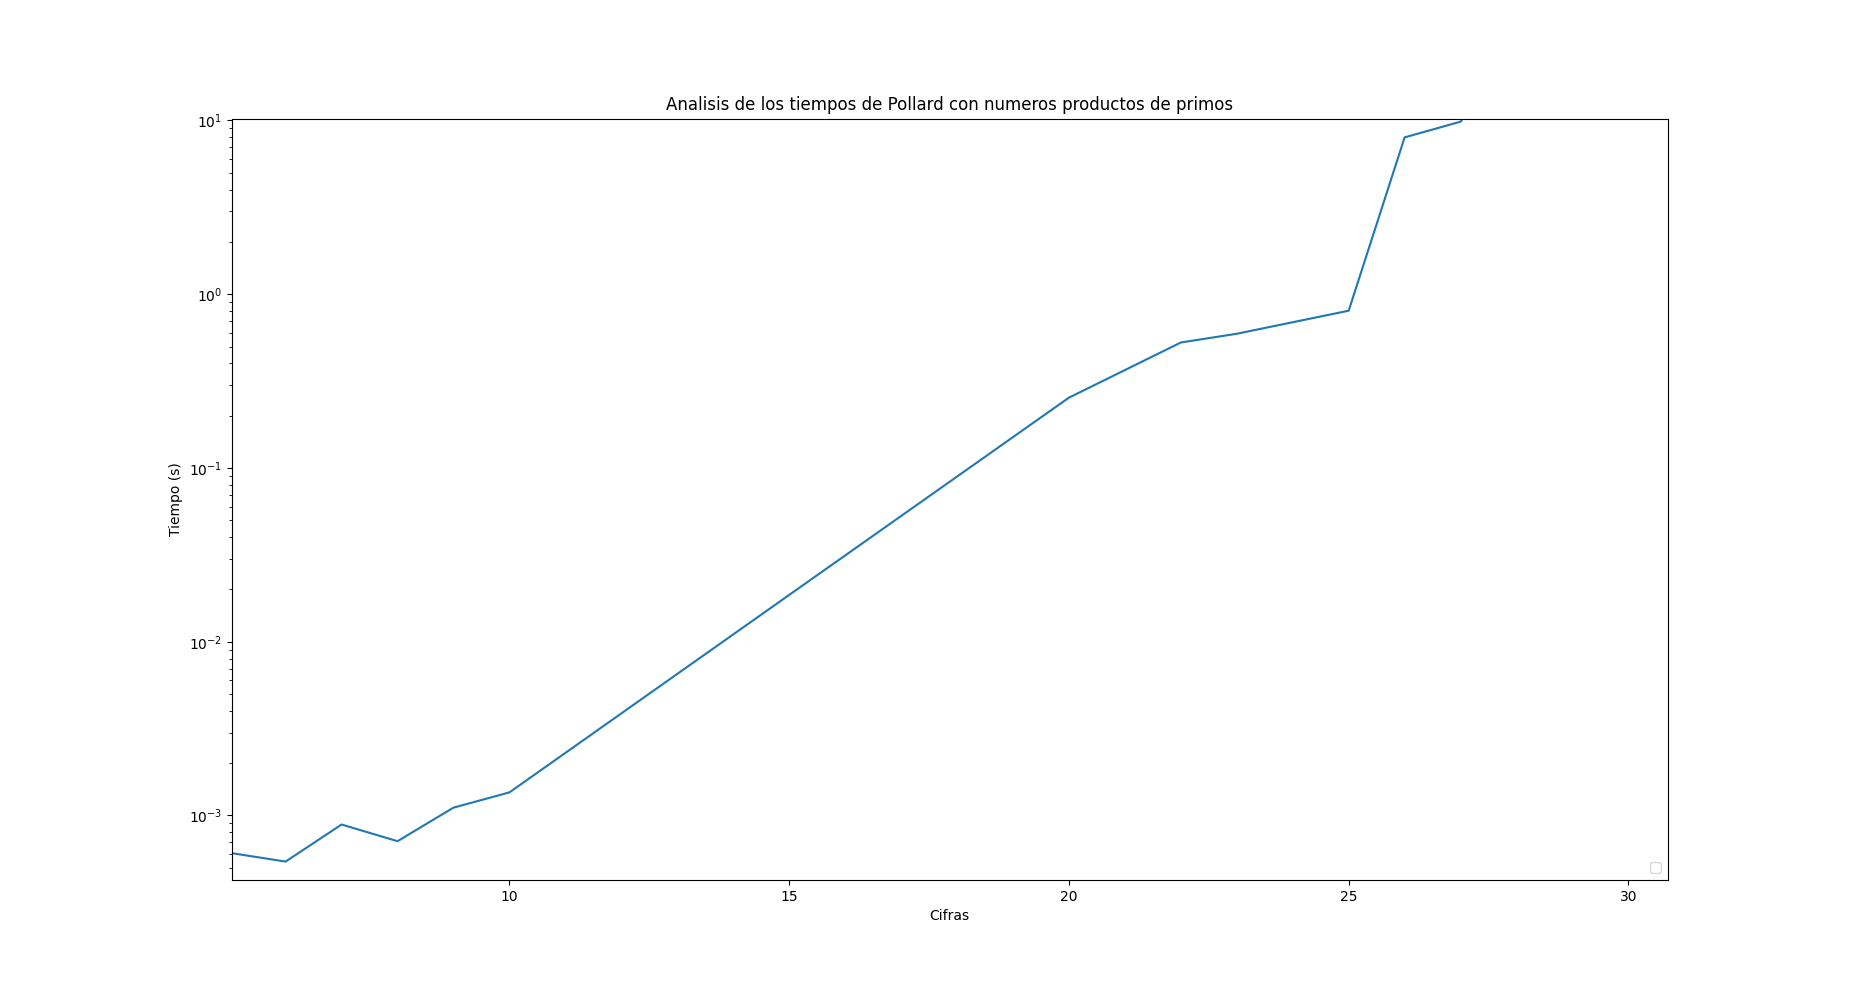
\includegraphics[scale=0.3]{Figure_6}
        \caption{Análisis de los tiempos de Pollard con números productos de dos primos}
        \label{fig:Figure_6}
    \end{figure}



\end{document}